\subsection{Infinite plate with a circular hole}
\paragraph{}
In this example, an infinite plate with a traction free hole under uniaxial tension $(\sigma = 1 N/m^2 )$
along x-axis (see Fig.~\ref{iso_fig:circular_hole_geo_bc}) is considered.

    \begin{figure}[h!]
        \centering
        \scalebox{0.5}{
            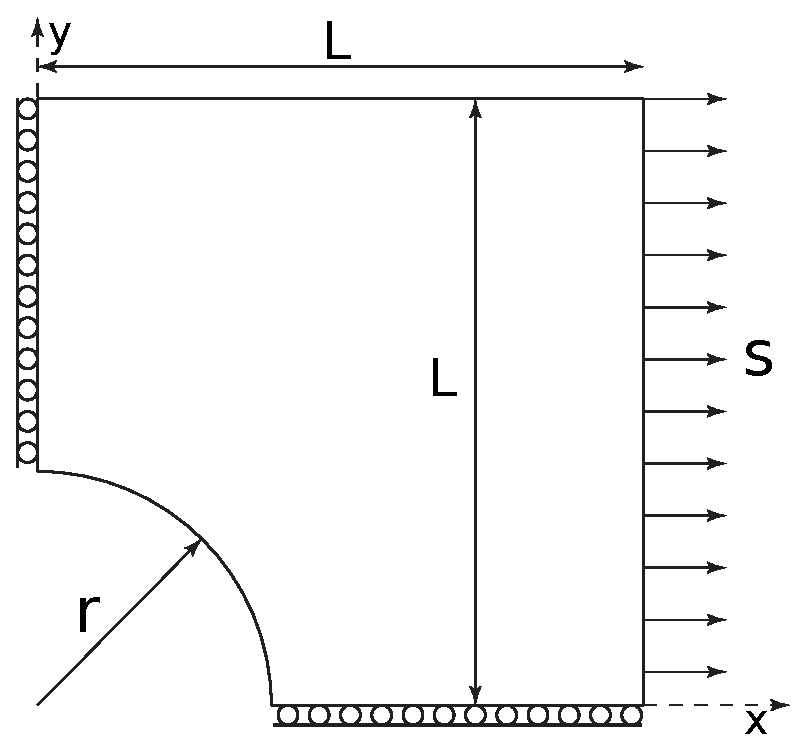
\includegraphics{isogeometric_sbfem/images/circular_hole_geo_bc.eps}
        }
        \caption{ Infinite plate with a circular hole: geometry and boundary conditions}
        \label{iso_fig:circular_hole_geo_bc}
    \end{figure}
%
The exact solution of the stresses in polar coordinate $(r,\theta)$ is given by \citep{Sukumar2001}:
    \begin{subequations}
        \begin{align}
            \sigma_{x}(r,\theta) &= 1 - \frac{a^2}{r^2} \left(
                \frac{3}{2} \cos2\theta +
                \cos4\theta
            \right) +
            \frac{3a^4}{2r^4} \cos4\theta\\
            \sigma_{y}(r,\theta) &= -\frac{a^2}{r^2} \left(
                \frac{1}{2} \cos2\theta -
                \cos4\theta
            \right) -
            \frac{3a^4}{2r^4} \cos4\theta\\
            \gamma_{xy}(r,\theta) &= -\frac{a^2}{r^2} \left(
                \frac{1}{2} \sin2\theta +
                \sin4\theta
            \right) -
            \frac{3a^4}{2r^4} \sin4\theta
        \end{align}
        \label{iso_eq:ex_chole_stress_sol}
    \end{subequations}
%
where $a$ is the radius of the hole.
Owing to symmetry, only one quarter of the plate is modeled.
% Fig. 10 shows a typical control net used for the study.
The material properties are: Young’s modulus $E = 100 N/m^2$ and Poisson’s ratio $\nu = 0.3$.
The closed form displacement in Cartesian coordinate is given as
    \begin{subequations}
        \begin{align}
            u_x(r,\theta) = \frac{R}{8G} \left[
                \frac{r}{R} (\kappa + 1) \cos\theta +
                2 \frac{R}{r} \left(
                    (1+ \kappa ) \cos\theta +
                    \cos3\theta
                \right) -
                2 \frac{R^3}{r^3}\cos3\theta
            \right] \\
            u_y(r,\theta) = \frac{R}{8G} \left[
                \frac{r}{R} (\kappa -3) \sin\theta +
                2 \frac{R}{r} \left(
                    (1 - \kappa) \sin\theta +
                    \sin3\theta
                \right) -
                2 \frac{R^3}{r^3}\sin3\theta
            \right]
        \end{align}
    \label{iso_eq:ex_chole_disp_sol}
    \end{subequations}
%
where $G$ is the shear modulus and $\kappa$ (Kolosov constant) is defined as
    \begin{equation}
        \kappa = \left\{
            \begin{aligned}   
                3-4 \nu \\
                \frac{3- \nu }{1+ \nu }    
            \end{aligned}
        \right.
    \label{iso_eq:kolosov_constant}
    \end{equation}
%
In this example, analytical tractions in Eq.~\ref{iso_eq:ex_chole_stress_sol} are applied on the boundary.
The left and bottom boundaries are constrained with a roller boundary condition. $u_x=0$ where $y=0$ and $u_y=0$ where $x=0$.

\paragraph{}
% result analysis
The convergence rate in terms of the displacement norm is shown in Fig.~\ref{iso_fig:circular_hole_convergence}
It is observed that the error decreases as the order of the shape functions is increased.
Another unique feature of the proposed method is that the method allows different type or order of shape functions to be employed for different segments of the boundary.
For example, in Fig.~\ref{iso_fig:circular_hole_mesh}, the arc A–B and the line segment B–C can be represented by different basis functions, i.e., the arc can be represented by NURBS and the line segment can be represented by conventional Lagrange basis functions.
Fig.~\ref{iso_fig:circular_hole_basis} shows the plot of the NURBS basis and Lagrange basis functions.
It can be seen that at point B, the shape function is continuous.
In order to assess the behavior, we represent the arc with quadratic NURBS and the straight lines with conventional Lagrange shape functions.
Since the NURBS are interpolatory at the ends, the compatibility requirement is automatically satisfied (see Fig.~\ref{iso_fig:circular_hole_shape_function_convergence}).
% The convergence of the relative error in the L 2 and H 1 is shown in Fig. 13.
The results from both the approaches converge with mesh refinement

    \begin{figure}
        \begin{subfigure}[b]{0.5\linewidth}
            \centering
            \scalebox{1}{
                % This file was created by matlab2tikz v0.4.6 running on MATLAB 8.0.
% Copyright (c) 2008--2014, Nico Schlömer <nico.schloemer@gmail.com>
% All rights reserved.
% Minimal pgfplots version: 1.3
% 
% The latest updates can be retrieved from
%   http://www.mathworks.com/matlabcentral/fileexchange/22022-matlab2tikz
% where you can also make suggestions and rate matlab2tikz.
% 
\begin{tikzpicture}[scale=0.6]

\begin{axis}[%
width=4.52083333333333in,
height=3.565625in,
scale only axis,
xmin=-0.197341513292434,
xmax=1.19734151329243,
ymin=-0.05,
ymax=1.05,
axis x line*=bottom,
axis y line*=left
]
\node[] at (-0.05,0.4) {$A$};
\node[] at (0.35,0) {$B$};
\addplot [color=blue,only marks,mark=o,mark options={solid},forget plot]
  table[row sep=crcr]{
0.6	0.6	\\
};
\label{archole_lab_sc}
\addplot [color=blue,dotted,mark size=4.2pt,mark=*,mark options={solid},forget plot]
  table[row sep=crcr]{
0.4	0	\\
0.4	0	\\
};
\label{archole_lab_cp}
\addplot [color=blue,dotted,mark size=4.2pt,mark=*,mark options={solid},forget plot]
  table[row sep=crcr]{
0.4	0	\\
0.7	0	\\
};
\addplot [color=blue,dotted,mark size=4.2pt,mark=*,mark options={solid},forget plot]
  table[row sep=crcr]{
0.7	0	\\
1	0	\\
};
\addplot [color=blue,dotted,mark size=4.2pt,mark=*,mark options={solid},forget plot]
  table[row sep=crcr]{
1	0	\\
1	0	\\
};
\addplot [color=blue,dotted,mark size=4.2pt,mark=*,mark options={solid},forget plot]
  table[row sep=crcr]{
1	0	\\
1	0.5	\\
};
\addplot [color=blue,dotted,mark size=4.2pt,mark=*,mark options={solid},forget plot]
  table[row sep=crcr]{
1	0.5	\\
1	1	\\
};
\addplot [color=blue,dotted,mark size=4.2pt,mark=*,mark options={solid},forget plot]
  table[row sep=crcr]{
1	1	\\
1	1	\\
};
\addplot [color=blue,dotted,mark size=4.2pt,mark=*,mark options={solid},forget plot]
  table[row sep=crcr]{
1	1	\\
0.5	1	\\
};
\addplot [color=blue,dotted,mark size=4.2pt,mark=*,mark options={solid},forget plot]
  table[row sep=crcr]{
0.5	1	\\
0	1	\\
};
\addplot [color=blue,dotted,mark size=4.2pt,mark=*,mark options={solid},forget plot]
  table[row sep=crcr]{
0	1	\\
0	1	\\
};
\addplot [color=blue,dotted,mark size=4.2pt,mark=*,mark options={solid},forget plot]
  table[row sep=crcr]{
0	1	\\
0	0.7	\\
};
\addplot [color=blue,dotted,mark size=4.2pt,mark=*,mark options={solid},forget plot]
  table[row sep=crcr]{
0	0.7	\\
0	0.4	\\
};
\addplot [color=blue,dotted,mark size=4.2pt,mark=*,mark options={solid},forget plot]
  table[row sep=crcr]{
0	0.4	\\
0	0.4	\\
};
\addplot [color=blue,dotted,mark size=4.2pt,mark=*,mark options={solid},forget plot]
  table[row sep=crcr]{
0	0.4	\\
0.4	0.4	\\
};
\addplot [color=blue,dotted,mark size=4.2pt,mark=*,mark options={solid},forget plot]
  table[row sep=crcr]{
0.4	0.4	\\
0.4	0	\\
};
\label{archole_lab_cpoly}
\addplot [color=blue,solid,forget plot]
  table[row sep=crcr]{
0	0.4	\\
0	1	\\
};
\label{archole_lab_mesh}
\addplot [color=blue,solid,forget plot]
  table[row sep=crcr]{
0	1	\\
1	1	\\
};
\addplot [color=blue,solid,forget plot]
  table[row sep=crcr]{
1	1	\\
1	0	\\
};
\addplot [color=blue,solid,forget plot]
  table[row sep=crcr]{
1	0	\\
0.4	0	\\
};
\addplot [color=blue,solid,forget plot]
  table[row sep=crcr]{
0.4	0	\\
0.399987538757663	0.00315734676388531	\\
0.399950155807063	0.00631449680545479	\\
0.399887853477391	0.0094712534146496	\\
0.39980063565047	0.0126274199059242	\\
0.39968850776051	0.0157827996305011	\\
0.399551476793777	0.0189371959886232	\\
0.399389551288152	0.0220904124418033	\\
0.399202741332597	0.0252422525250695	\\
0.398991058566535	0.0283925198592064	\\
0.398754516179117	0.0315410181629906	\\
0.398493128908403	0.0346875512654203	\\
0.398206913040442	0.037831923117938	\\
0.397895886408263	0.0409739378066453	\\
0.397560068390755	0.04411339956451	\\
0.397199479911468	0.0472501127835632	\\
0.396814143437303	0.050383882027087	\\
0.396404082977117	0.0535145120417917	\\
0.395969324080223	0.0566418077699807	\\
0.395509893834801	0.0597655743617044	\\
0.39502582086621	0.0628856171869003	\\
0.394517135335201	0.0660017418475197	\\
0.393983868936044	0.0691137541896398	\\
0.393426054894548	0.0722214603155609	\\
0.392843727965992	0.0753246665958872	\\
0.392236924432962	0.0784231796815912	\\
0.391605682103086	0.0815168065160609	\\
0.390950040306683	0.0846053543471276	\\
0.390270039894309	0.0876886307390765	\\
0.389565723234215	0.0907664435846361	\\
0.388837134209703	0.0938386011169475	\\
0.388084318216395	0.0969049119215133	\\
0.387307322159403	0.0999651849481233	\\
0.386506194450409	0.103019229522759	\\
0.385680985004645	0.106066855359471	\\
0.384831745237785	0.109107872572241	\\
0.383958528062743	0.112142091686806	\\
0.383061387886372	0.115169323652467	\\
0.382140380606078	0.118189379853868	\\
0.381195563606336	0.121202072122749	\\
0.380226995755113	0.124207212749668	\\
0.379234737400204	0.127204614495695	\\
0.378218850365467	0.130194090604085	\\
0.377179397946975	0.133175454811904	\\
0.37611644490907	0.136148521361645	\\
0.37503005748033	0.139113105012793	\\
0.373920303349439	0.142069021053371	\\
0.372787251660974	0.14501608531145	\\
0.371630973011092	0.147954114166619	\\
0.370451539443136	0.15088292456143	\\
0.369249024443144	0.153802334012804	\\
0.36802350293527	0.156712160623397	\\
0.366775051277116	0.159612223092936	\\
0.365503747254975	0.162502340729516	\\
0.364209670078985	0.165382333460854	\\
0.362892900378193	0.168252021845514	\\
0.361553520195529	0.171111227084084	\\
0.360191612982701	0.173959771030317	\\
0.358807263594985	0.176797476202232	\\
0.35740055828595	0.179624165793168	\\
0.355971584702072	0.182439663682806	\\
0.354520431877283	0.185243794448139	\\
0.353047190227419	0.188036383374401	\\
0.351551951544584	0.190817256465956	\\
0.350034808991438	0.193586240457136	\\
0.348495857095384	0.196343162823037	\\
0.346935191742686	0.199087851790273	\\
0.345352910172489	0.201820136347671	\\
0.343749110970765	0.204539846256931	\\
0.342123894064165	0.207246812063231	\\
0.340477360713798	0.209940865105787	\\
0.33880961350892	0.212621837528361	\\
0.33712075636054	0.215289562289715	\\
0.335410894494951	0.217943873174028	\\
0.333680134447167	0.220584604801243	\\
0.33192858405429	0.223211592637376	\\
0.33015635244879	0.225824673004767	\\
0.328363550051705	0.228423683092278	\\
0.32655028856576	0.231008460965435	\\
0.324716680968408	0.233578845576523	\\
0.322862841504794	0.236134676774611	\\
0.320988885680631	0.238675795315542	\\
0.319094930255008	0.241202042871846	\\
0.317181093233111	0.243713262042607	\\
0.315247493858877	0.246209296363272	\\
0.313294252607556	0.248689990315398	\\
0.311321491178212	0.251155189336343	\\
0.309329332486136	0.253604739828895	\\
0.307317900655188	0.256038489170843	\\
0.305287321010067	0.258456285724484	\\
0.303237720068498	0.260857978846075	\\
0.301169225533351	0.263243418895215	\\
0.299081966284684	0.265612457244172	\\
0.296976072371713	0.267964946287142	\\
0.294851675004712	0.270300739449443	\\
0.292708906546831	0.272619691196654	\\
0.290547900505856	0.274921657043674	\\
0.288368791525887	0.277206493563733	\\
0.286171715378949	0.279474058397323	\\
0.283956808956533	0.281724210261069	\\
0.281724210261069	0.283956808956533	\\
0.279474058397323	0.286171715378949	\\
0.277206493563733	0.288368791525887	\\
0.274921657043674	0.290547900505856	\\
0.272619691196654	0.292708906546831	\\
0.270300739449443	0.294851675004712	\\
0.267964946287142	0.296976072371713	\\
0.265612457244173	0.299081966284684	\\
0.263243418895215	0.301169225533351	\\
0.260857978846075	0.303237720068498	\\
0.258456285724484	0.305287321010067	\\
0.256038489170843	0.307317900655188	\\
0.253604739828895	0.309329332486136	\\
0.251155189336343	0.311321491178212	\\
0.248689990315398	0.313294252607556	\\
0.246209296363272	0.315247493858877	\\
0.243713262042607	0.317181093233111	\\
0.241202042871846	0.319094930255008	\\
0.238675795315542	0.320988885680631	\\
0.236134676774611	0.322862841504794	\\
0.233578845576523	0.324716680968408	\\
0.231008460965435	0.32655028856576	\\
0.228423683092278	0.328363550051705	\\
0.225824673004767	0.33015635244879	\\
0.223211592637376	0.33192858405429	\\
0.220584604801243	0.333680134447167	\\
0.217943873174028	0.335410894494951	\\
0.215289562289715	0.33712075636054	\\
0.212621837528361	0.33880961350892	\\
0.209940865105787	0.340477360713798	\\
0.207246812063231	0.342123894064165	\\
0.204539846256931	0.343749110970765	\\
0.201820136347671	0.345352910172489	\\
0.199087851790273	0.346935191742686	\\
0.196343162823038	0.348495857095384	\\
0.193586240457136	0.350034808991437	\\
0.190817256465956	0.351551951544584	\\
0.188036383374401	0.353047190227419	\\
0.185243794448139	0.354520431877283	\\
0.182439663682806	0.355971584702072	\\
0.179624165793168	0.35740055828595	\\
0.176797476202232	0.358807263594985	\\
0.173959771030317	0.360191612982701	\\
0.171111227084084	0.361553520195529	\\
0.168252021845514	0.362892900378193	\\
0.165382333460854	0.364209670078985	\\
0.162502340729516	0.365503747254975	\\
0.159612223092936	0.366775051277116	\\
0.156712160623397	0.36802350293527	\\
0.153802334012804	0.369249024443144	\\
0.15088292456143	0.370451539443136	\\
0.147954114166619	0.371630973011092	\\
0.14501608531145	0.372787251660974	\\
0.142069021053371	0.373920303349439	\\
0.139113105012793	0.37503005748033	\\
0.136148521361645	0.37611644490907	\\
0.133175454811905	0.377179397946975	\\
0.130194090604085	0.378218850365467	\\
0.127204614495695	0.379234737400204	\\
0.124207212749668	0.380226995755113	\\
0.121202072122749	0.381195563606336	\\
0.118189379853868	0.382140380606078	\\
0.115169323652467	0.383061387886372	\\
0.112142091686806	0.383958528062743	\\
0.109107872572241	0.384831745237785	\\
0.106066855359472	0.385680985004645	\\
0.103019229522759	0.386506194450409	\\
0.0999651849481234	0.387307322159403	\\
0.0969049119215133	0.388084318216395	\\
0.0938386011169475	0.388837134209703	\\
0.0907664435846361	0.389565723234215	\\
0.0876886307390766	0.390270039894309	\\
0.0846053543471276	0.390950040306683	\\
0.0815168065160609	0.391605682103086	\\
0.0784231796815913	0.392236924432962	\\
0.0753246665958872	0.392843727965992	\\
0.0722214603155609	0.393426054894548	\\
0.0691137541896398	0.393983868936044	\\
0.0660017418475197	0.394517135335201	\\
0.0628856171869003	0.39502582086621	\\
0.0597655743617044	0.395509893834801	\\
0.0566418077699807	0.395969324080223	\\
0.0535145120417917	0.396404082977117	\\
0.0503838820270871	0.396814143437303	\\
0.0472501127835632	0.397199479911468	\\
0.0441133995645101	0.397560068390755	\\
0.0409739378066454	0.397895886408263	\\
0.037831923117938	0.398206913040442	\\
0.0346875512654203	0.398493128908403	\\
0.0315410181629906	0.398754516179117	\\
0.0283925198592064	0.398991058566535	\\
0.0252422525250695	0.399202741332597	\\
0.0220904124418033	0.399389551288152	\\
0.0189371959886233	0.399551476793777	\\
0.0157827996305011	0.39968850776051	\\
0.0126274199059243	0.39980063565047	\\
0.00947125341464964	0.399887853477391	\\
0.00631449680545488	0.399950155807063	\\
0.00315734676388529	0.399987538757663	\\
2.44929359829471e-17	0.4	\\
};
\end{axis}
\end{tikzpicture}%
            }            
        \end{subfigure}
        \begin{subfigure}[b]{0.5\linewidth}
            \centering
            \scalebox{1}{
                % This file was created by matlab2tikz v0.4.6 running on MATLAB 8.0.
% Copyright (c) 2008--2014, Nico Schlömer <nico.schloemer@gmail.com>
% All rights reserved.
% Minimal pgfplots version: 1.3
% 
% The latest updates can be retrieved from
%   http://www.mathworks.com/matlabcentral/fileexchange/22022-matlab2tikz
% where you can also make suggestions and rate matlab2tikz.
% 
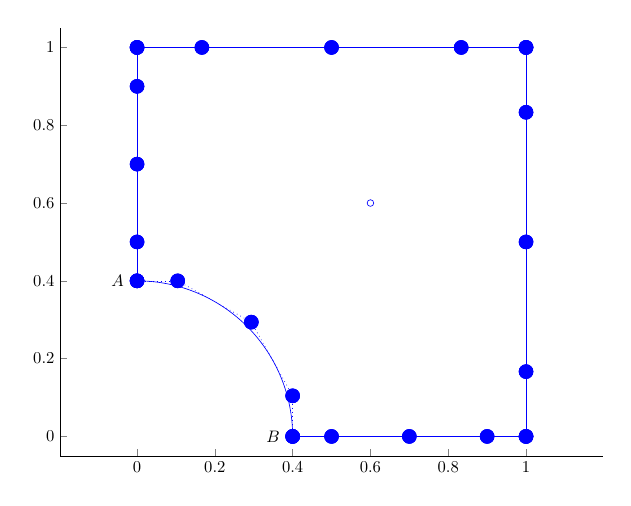
\begin{tikzpicture}[scale=0.6]

\begin{axis}[%
width=4.52083333333333in,
height=3.565625in,
scale only axis,
xmin=-0.197341513292434,
xmax=1.19734151329243,
ymin=-0.05,
ymax=1.05,
axis x line*=bottom,
axis y line*=left
]
\node[] at (-0.05,0.4) {$A$};
\node[] at (0.35,0) {$B$};
\addplot [color=blue,only marks,mark=o,mark options={solid},forget plot]
  table[row sep=crcr]{
0.6	0.6	\\
};
\addplot [color=blue,dotted,mark size=4.2pt,mark=*,mark options={solid},forget plot]
  table[row sep=crcr]{
0.4	0	\\
0.4	0	\\
};
\addplot [color=blue,dotted,mark size=4.2pt,mark=*,mark options={solid},forget plot]
  table[row sep=crcr]{
0.4	0	\\
0.5	0	\\
};
\addplot [color=blue,dotted,mark size=4.2pt,mark=*,mark options={solid},forget plot]
  table[row sep=crcr]{
0.5	0	\\
0.7	0	\\
};
\addplot [color=blue,dotted,mark size=4.2pt,mark=*,mark options={solid},forget plot]
  table[row sep=crcr]{
0.7	0	\\
0.9	1.11022302462516e-16	\\
};
\addplot [color=blue,dotted,mark size=4.2pt,mark=*,mark options={solid},forget plot]
  table[row sep=crcr]{
0.9	1.11022302462516e-16	\\
1	0	\\
};
\addplot [color=blue,dotted,mark size=4.2pt,mark=*,mark options={solid},forget plot]
  table[row sep=crcr]{
1	0	\\
1	0	\\
};
\addplot [color=blue,dotted,mark size=4.2pt,mark=*,mark options={solid},forget plot]
  table[row sep=crcr]{
1	0	\\
1	0.166666666666667	\\
};
\addplot [color=blue,dotted,mark size=4.2pt,mark=*,mark options={solid},forget plot]
  table[row sep=crcr]{
1	0.166666666666667	\\
1	0.5	\\
};
\addplot [color=blue,dotted,mark size=4.2pt,mark=*,mark options={solid},forget plot]
  table[row sep=crcr]{
1	0.5	\\
1	0.833333333333333	\\
};
\addplot [color=blue,dotted,mark size=4.2pt,mark=*,mark options={solid},forget plot]
  table[row sep=crcr]{
1	0.833333333333333	\\
1	1	\\
};
\addplot [color=blue,dotted,mark size=4.2pt,mark=*,mark options={solid},forget plot]
  table[row sep=crcr]{
1	1	\\
1	1	\\
};
\addplot [color=blue,dotted,mark size=4.2pt,mark=*,mark options={solid},forget plot]
  table[row sep=crcr]{
1	1	\\
0.833333333333333	1	\\
};
\addplot [color=blue,dotted,mark size=4.2pt,mark=*,mark options={solid},forget plot]
  table[row sep=crcr]{
0.833333333333333	1	\\
0.5	1	\\
};
\addplot [color=blue,dotted,mark size=4.2pt,mark=*,mark options={solid},forget plot]
  table[row sep=crcr]{
0.5	1	\\
0.166666666666667	1	\\
};
\addplot [color=blue,dotted,mark size=4.2pt,mark=*,mark options={solid},forget plot]
  table[row sep=crcr]{
0.166666666666667	1	\\
0	1	\\
};
\addplot [color=blue,dotted,mark size=4.2pt,mark=*,mark options={solid},forget plot]
  table[row sep=crcr]{
0	1	\\
0	1	\\
};
\addplot [color=blue,dotted,mark size=4.2pt,mark=*,mark options={solid},forget plot]
  table[row sep=crcr]{
0	1	\\
0	0.9	\\
};
\addplot [color=blue,dotted,mark size=4.2pt,mark=*,mark options={solid},forget plot]
  table[row sep=crcr]{
0	0.9	\\
0	0.7	\\
};
\addplot [color=blue,dotted,mark size=4.2pt,mark=*,mark options={solid},forget plot]
  table[row sep=crcr]{
0	0.7	\\
1.11022302462516e-16	0.5	\\
};
\addplot [color=blue,dotted,mark size=4.2pt,mark=*,mark options={solid},forget plot]
  table[row sep=crcr]{
1.11022302462516e-16	0.5	\\
0	0.4	\\
};
\addplot [color=blue,dotted,mark size=4.2pt,mark=*,mark options={solid},forget plot]
  table[row sep=crcr]{
0	0.4	\\
0	0.4	\\
};
\addplot [color=blue,dotted,mark size=4.2pt,mark=*,mark options={solid},forget plot]
  table[row sep=crcr]{
0	0.4	\\
0.104481549985497	0.4	\\
};
\addplot [color=blue,dotted,mark size=4.2pt,mark=*,mark options={solid},forget plot]
  table[row sep=crcr]{
0.104481549985497	0.4	\\
0.293836321356054	0.293836321356054	\\
};
\addplot [color=blue,dotted,mark size=4.2pt,mark=*,mark options={solid},forget plot]
  table[row sep=crcr]{
0.293836321356054	0.293836321356054	\\
0.4	0.104481549985497	\\
};
\addplot [color=blue,dotted,mark size=4.2pt,mark=*,mark options={solid},forget plot]
  table[row sep=crcr]{
0.4	0.104481549985497	\\
0.4	0	\\
};
\addplot [color=blue,solid,forget plot]
  table[row sep=crcr]{
0	0.4	\\
0	1	\\
};
\addplot [color=blue,solid,forget plot]
  table[row sep=crcr]{
0	1	\\
1	1	\\
};
\addplot [color=blue,solid,forget plot]
  table[row sep=crcr]{
1	1	\\
1	0	\\
};
\addplot [color=blue,solid,forget plot]
  table[row sep=crcr]{
1	0	\\
0.4	0	\\
};
\addplot [color=blue,solid,forget plot]
  table[row sep=crcr]{
0.4	0	\\
0.399987538757663	0.00315734676388531	\\
0.399950155807063	0.00631449680545479	\\
0.399887853477391	0.0094712534146496	\\
0.39980063565047	0.0126274199059242	\\
0.39968850776051	0.0157827996305011	\\
0.399551476793777	0.0189371959886232	\\
0.399389551288152	0.0220904124418033	\\
0.399202741332597	0.0252422525250695	\\
0.398991058566535	0.0283925198592064	\\
0.398754516179117	0.0315410181629906	\\
0.398493128908403	0.0346875512654203	\\
0.398206913040442	0.037831923117938	\\
0.397895886408263	0.0409739378066453	\\
0.397560068390755	0.04411339956451	\\
0.397199479911468	0.0472501127835632	\\
0.396814143437303	0.050383882027087	\\
0.396404082977117	0.0535145120417917	\\
0.395969324080223	0.0566418077699807	\\
0.395509893834801	0.0597655743617044	\\
0.39502582086621	0.0628856171869003	\\
0.394517135335201	0.0660017418475197	\\
0.393983868936044	0.0691137541896398	\\
0.393426054894548	0.0722214603155609	\\
0.392843727965992	0.0753246665958872	\\
0.392236924432962	0.0784231796815912	\\
0.391605682103086	0.0815168065160609	\\
0.390950040306683	0.0846053543471276	\\
0.390270039894309	0.0876886307390765	\\
0.389565723234215	0.0907664435846361	\\
0.388837134209703	0.0938386011169475	\\
0.388084318216395	0.0969049119215133	\\
0.387307322159403	0.0999651849481233	\\
0.386506194450409	0.103019229522759	\\
0.385680985004645	0.106066855359471	\\
0.384831745237785	0.109107872572241	\\
0.383958528062743	0.112142091686806	\\
0.383061387886372	0.115169323652467	\\
0.382140380606078	0.118189379853868	\\
0.381195563606336	0.121202072122749	\\
0.380226995755113	0.124207212749668	\\
0.379234737400204	0.127204614495695	\\
0.378218850365467	0.130194090604085	\\
0.377179397946975	0.133175454811904	\\
0.37611644490907	0.136148521361645	\\
0.37503005748033	0.139113105012793	\\
0.373920303349439	0.142069021053371	\\
0.372787251660974	0.14501608531145	\\
0.371630973011092	0.147954114166619	\\
0.370451539443136	0.15088292456143	\\
0.369249024443144	0.153802334012804	\\
0.36802350293527	0.156712160623397	\\
0.366775051277116	0.159612223092936	\\
0.365503747254975	0.162502340729516	\\
0.364209670078985	0.165382333460854	\\
0.362892900378193	0.168252021845514	\\
0.361553520195529	0.171111227084084	\\
0.360191612982701	0.173959771030317	\\
0.358807263594985	0.176797476202232	\\
0.35740055828595	0.179624165793168	\\
0.355971584702072	0.182439663682806	\\
0.354520431877283	0.185243794448139	\\
0.353047190227419	0.188036383374401	\\
0.351551951544584	0.190817256465956	\\
0.350034808991438	0.193586240457136	\\
0.348495857095384	0.196343162823037	\\
0.346935191742686	0.199087851790273	\\
0.345352910172489	0.201820136347671	\\
0.343749110970765	0.204539846256931	\\
0.342123894064165	0.207246812063231	\\
0.340477360713798	0.209940865105787	\\
0.33880961350892	0.212621837528361	\\
0.33712075636054	0.215289562289715	\\
0.335410894494951	0.217943873174028	\\
0.333680134447167	0.220584604801243	\\
0.33192858405429	0.223211592637376	\\
0.33015635244879	0.225824673004767	\\
0.328363550051705	0.228423683092278	\\
0.32655028856576	0.231008460965435	\\
0.324716680968408	0.233578845576523	\\
0.322862841504794	0.236134676774611	\\
0.320988885680631	0.238675795315542	\\
0.319094930255008	0.241202042871846	\\
0.317181093233111	0.243713262042607	\\
0.315247493858877	0.246209296363272	\\
0.313294252607556	0.248689990315398	\\
0.311321491178212	0.251155189336343	\\
0.309329332486136	0.253604739828895	\\
0.307317900655188	0.256038489170843	\\
0.305287321010067	0.258456285724484	\\
0.303237720068498	0.260857978846075	\\
0.301169225533351	0.263243418895215	\\
0.299081966284684	0.265612457244172	\\
0.296976072371713	0.267964946287142	\\
0.294851675004712	0.270300739449443	\\
0.292708906546831	0.272619691196654	\\
0.290547900505856	0.274921657043674	\\
0.288368791525887	0.277206493563733	\\
0.286171715378949	0.279474058397323	\\
0.283956808956533	0.281724210261069	\\
0.281724210261069	0.283956808956533	\\
0.279474058397323	0.286171715378949	\\
0.277206493563733	0.288368791525887	\\
0.274921657043674	0.290547900505856	\\
0.272619691196654	0.292708906546831	\\
0.270300739449443	0.294851675004712	\\
0.267964946287142	0.296976072371713	\\
0.265612457244173	0.299081966284684	\\
0.263243418895215	0.301169225533351	\\
0.260857978846075	0.303237720068498	\\
0.258456285724484	0.305287321010067	\\
0.256038489170843	0.307317900655188	\\
0.253604739828895	0.309329332486136	\\
0.251155189336343	0.311321491178212	\\
0.248689990315398	0.313294252607556	\\
0.246209296363272	0.315247493858877	\\
0.243713262042607	0.317181093233111	\\
0.241202042871846	0.319094930255008	\\
0.238675795315542	0.320988885680631	\\
0.236134676774611	0.322862841504794	\\
0.233578845576523	0.324716680968408	\\
0.231008460965435	0.32655028856576	\\
0.228423683092278	0.328363550051705	\\
0.225824673004767	0.33015635244879	\\
0.223211592637376	0.33192858405429	\\
0.220584604801243	0.333680134447167	\\
0.217943873174028	0.335410894494951	\\
0.215289562289715	0.33712075636054	\\
0.212621837528361	0.33880961350892	\\
0.209940865105787	0.340477360713798	\\
0.207246812063231	0.342123894064165	\\
0.204539846256931	0.343749110970765	\\
0.201820136347671	0.345352910172489	\\
0.199087851790273	0.346935191742686	\\
0.196343162823038	0.348495857095384	\\
0.193586240457136	0.350034808991437	\\
0.190817256465956	0.351551951544584	\\
0.188036383374401	0.353047190227419	\\
0.185243794448139	0.354520431877283	\\
0.182439663682806	0.355971584702072	\\
0.179624165793168	0.35740055828595	\\
0.176797476202232	0.358807263594985	\\
0.173959771030317	0.360191612982701	\\
0.171111227084084	0.361553520195529	\\
0.168252021845514	0.362892900378193	\\
0.165382333460854	0.364209670078985	\\
0.162502340729516	0.365503747254975	\\
0.159612223092936	0.366775051277116	\\
0.156712160623397	0.36802350293527	\\
0.153802334012804	0.369249024443144	\\
0.15088292456143	0.370451539443136	\\
0.147954114166619	0.371630973011092	\\
0.14501608531145	0.372787251660974	\\
0.142069021053371	0.373920303349439	\\
0.139113105012793	0.37503005748033	\\
0.136148521361645	0.37611644490907	\\
0.133175454811905	0.377179397946975	\\
0.130194090604085	0.378218850365467	\\
0.127204614495695	0.379234737400204	\\
0.124207212749668	0.380226995755113	\\
0.121202072122749	0.381195563606336	\\
0.118189379853868	0.382140380606078	\\
0.115169323652467	0.383061387886372	\\
0.112142091686806	0.383958528062743	\\
0.109107872572241	0.384831745237785	\\
0.106066855359472	0.385680985004645	\\
0.103019229522759	0.386506194450409	\\
0.0999651849481234	0.387307322159403	\\
0.0969049119215133	0.388084318216395	\\
0.0938386011169475	0.388837134209703	\\
0.0907664435846361	0.389565723234215	\\
0.0876886307390766	0.390270039894309	\\
0.0846053543471276	0.390950040306683	\\
0.0815168065160609	0.391605682103086	\\
0.0784231796815913	0.392236924432962	\\
0.0753246665958872	0.392843727965992	\\
0.0722214603155609	0.393426054894548	\\
0.0691137541896398	0.393983868936044	\\
0.0660017418475197	0.394517135335201	\\
0.0628856171869003	0.39502582086621	\\
0.0597655743617044	0.395509893834801	\\
0.0566418077699807	0.395969324080223	\\
0.0535145120417917	0.396404082977117	\\
0.0503838820270871	0.396814143437303	\\
0.0472501127835632	0.397199479911468	\\
0.0441133995645101	0.397560068390755	\\
0.0409739378066454	0.397895886408263	\\
0.037831923117938	0.398206913040442	\\
0.0346875512654203	0.398493128908403	\\
0.0315410181629906	0.398754516179117	\\
0.0283925198592064	0.398991058566535	\\
0.0252422525250695	0.399202741332597	\\
0.0220904124418033	0.399389551288152	\\
0.0189371959886233	0.399551476793777	\\
0.0157827996305011	0.39968850776051	\\
0.0126274199059243	0.39980063565047	\\
0.00947125341464964	0.399887853477391	\\
0.00631449680545488	0.399950155807063	\\
0.00315734676388529	0.399987538757663	\\
2.44929359829471e-17	0.4	\\
};
\end{axis}
\end{tikzpicture}%
            }
        \end{subfigure}
        \caption[Plate with circular hole: mesh]{
            Plate with circular hole: control net for two different discretizations.
            Control points ( 
                \tikz\draw[blue,fill=blue] (0,0) circle (.7ex);
            ), Boundary lines (
                \tikz[baseline=-0.5ex]\draw[blue,thick] (0,0) -- (0.5,0);
            ), Control polygon (
                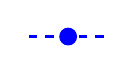
\begin{tikzpicture}[baseline=-0.5ex]
                    \draw[blue,thick,dashed] (0,0) -- (1,0);
                    \draw[blue,fill=blue] (0.5,0) circle (.7ex);
                \end{tikzpicture}
            ),
            Scaling center (
                \tikz[baseline=-0.5ex]\draw[blue] (0,0) circle (0.7ex);
            ).
        }
    \label{iso_fig:circular_hole_mesh}
    \end{figure}

    \begin{figure}
        \begin{subfigure}[b]{1\linewidth}
            \centering
            \scalebox{0.7}{
                % This file was created by matlab2tikz v0.4.6 running on MATLAB 8.2.
% Copyright (c) 2008--2014, Nico Schlömer <nico.schloemer@gmail.com>
% All rights reserved.
% Minimal pgfplots version: 1.3
% 
% The latest updates can be retrieved from
%   http://www.mathworks.com/matlabcentral/fileexchange/22022-matlab2tikz
% where you can also make suggestions and rate matlab2tikz.
% 
%
% defining custom colors
\definecolor{mycolor1}{rgb}{0.00000,0.75000,0.75000}%
\definecolor{mycolor2}{rgb}{0.75000,0.00000,0.75000}%
%
\begin{tikzpicture}

\begin{axis}[%
width=4.52083333333333in,
height=3.5146875in,
scale only axis,
xmode=log,
xmin=10,
xmax=1000,
xminorticks=true,
xlabel={Total DOF},
ymode=log,
ymin=1e-09,
ymax=0.1,
yminorticks=true,
ylabel={Error},
title={L2L Displacement Error},
legend style={draw=black,fill=white,legend cell align=left}
]
\addplot [color=blue,solid,mark=square,mark options={solid}]
  table[row sep=crcr]{
20	0.052647009	\\
40	0.015077369	\\
80	0.004598634	\\
160	0.001317239	\\
};
\addlegendentry{1st order};

\addplot [color=black!50!green,solid,mark=o,mark options={solid}]
  table[row sep=crcr]{
20	0.018330302	\\
40	0.000979438	\\
80	9.0447e-05	\\
160	7.10192e-06	\\
};
\addlegendentry{2nd order};

\addplot [color=red,solid,mark=triangle,mark options={solid,,rotate=180}]
  table[row sep=crcr]{
40	0.001028186	\\
80	6.4874e-06	\\
160	9.03877e-08	\\
};
\addlegendentry{4th order};

\addplot [color=mycolor1,solid,mark=asterisk,mark options={solid}]
  table[row sep=crcr]{
80	8.12048e-06	\\
160	7.13386e-09	\\
};
\addlegendentry{6th order};

\addplot [color=mycolor2,solid,mark=+,mark options={solid}]
  table[row sep=crcr]{
20	0.0371	\\
40	0.00228	\\
80	0.000316	\\
160	2.98e-05	\\
};
\addlegendentry{LNGL 2nd order};

\end{axis}
\end{tikzpicture}%
            }
            \label{iso_fig:circular_hole_displacement_convergence}
            \caption{the relative error in displacement norm $(L^2)$}
        \end{subfigure}
        
        \begin{subfigure}[b]{1\linewidth}
            \centering
            \scalebox{0.7}{
                % This file was created by matlab2tikz v0.4.6 running on MATLAB 8.2.
% Copyright (c) 2008--2014, Nico Schlömer <nico.schloemer@gmail.com>
% All rights reserved.
% Minimal pgfplots version: 1.3
% 
% The latest updates can be retrieved from
%   http://www.mathworks.com/matlabcentral/fileexchange/22022-matlab2tikz
% where you can also make suggestions and rate matlab2tikz.
% 
%
% defining custom colors
\definecolor{mycolor1}{rgb}{0.00000,0.75000,0.75000}%
\definecolor{mycolor2}{rgb}{0.75000,0.00000,0.75000}%
%
\begin{tikzpicture}

\begin{axis}[%
width=4.52083333333333in,
height=3.5146875in,
scale only axis,
xmode=log,
xmin=10,
xmax=1000,
xminorticks=true,
xlabel={Total DOF},
ymode=log,
ymin=1e-05,
ymax=1,
yminorticks=true,
ylabel={Error},
title={L2L Strain Energy Error},
legend style={draw=black,fill=white,legend cell align=left}
]
\addplot [color=blue,solid,mark=square,mark options={solid}]
  table[row sep=crcr]{
20	0.136951345	\\
40	0.070082184	\\
80	0.040238511	\\
160	0.02076975	\\
};
\addlegendentry{1st order};

\addplot [color=black!50!green,solid,mark=o,mark options={solid}]
  table[row sep=crcr]{
20	0.115220087	\\
40	0.0192672307117524	\\
80	0.002314805	\\
160	0.000499173	\\
};
\addlegendentry{2nd order};

\addplot [color=red,solid,mark=triangle,mark options={solid,,rotate=180}]
  table[row sep=crcr]{
40	0.028460196	\\
80	0.001326623	\\
160	6.43781e-05	\\
};
\addlegendentry{4th order};

\addplot [color=mycolor1,solid,mark=asterisk,mark options={solid}]
  table[row sep=crcr]{
80	0.000931962	\\
160	1.04862e-05	\\
};
\addlegendentry{6th order};

\addplot [color=mycolor2,solid,mark=+,mark options={solid}]
  table[row sep=crcr]{
20	0.196598384	\\
40	0.040130929	\\
80	0.00697	\\
160	0.00196	\\
};
\addlegendentry{LNGL 2nd order};

\end{axis}
\end{tikzpicture}%
            }
            \label{iso_fig:circular_hole_energy_convergence}
            \caption{the relative error in the energy norm}
        \end{subfigure}
    \caption{Bending of thick cantilever beam: Convergence results}
    \label{iso_fig:circular_hole_convergence}
    \end{figure}

    \begin{figure}
        \centering
        \scalebox{0.5}{
            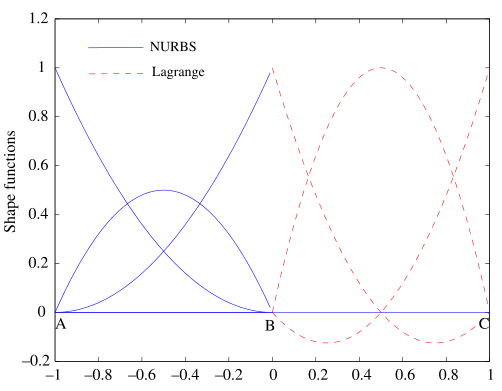
\includegraphics{isogeometric_sbfem/images/circular_hole_basis.png}
        }
        \caption{NURBS basis functions and Lagrange basis functions. It can be seen that at Point $B$, the shape functions are continuous}
        \label{iso_fig:circular_hole_basis}
    \end{figure}

    \begin{figure}
        \centering
        \scalebox{0.5}{
            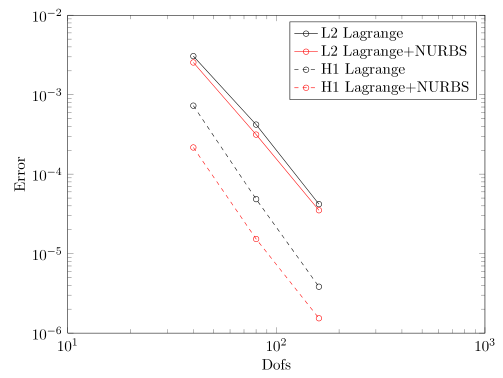
\includegraphics{isogeometric_sbfem/images/circular_hole_shape_function_convergence.png}
        }
        \caption{
            Infinite plate with a circular hole: Convergence results for the relative error in the displacement norm ($L^2$) and
                the relative error in the energy norm. In this case, the arc is represented with NURBS and Lagrange shape functions.
        }
        \label{iso_fig:circular_hole_shape_function_convergence}
    \end{figure}

\pagebreak